\documentclass[twocolumn,superscriptaddress,aps]{revtex4-1}

\usepackage[utf8]{inputenc}

\usepackage{amsfonts}
\usepackage{amssymb}
\usepackage{amsmath}
\usepackage{amsthm}

\usepackage{bm}
\usepackage{cancel}
\usepackage{bbold}
\usepackage{slashed}
\usepackage{graphicx}
\usepackage{color}
\usepackage{hyperref}
\usepackage{algorithm}
\usepackage{algpseudocode}
\usepackage{tikz}

\newcommand{\glnote}[1]{\textcolor{red}{[GL: #1]}}
\newcommand{\kcnote}[1]{\textcolor{red}{[KC: #1]}}

\theoremstyle{plain}
\newtheorem{theorem}{Theorem}
\newtheorem{proposition}[theorem]{Proposition}

\begin{document}


% ==============================================================================

\title{\Large{Adversarial Variational Optimization of Non-Differentiable Simulators}}
\vspace{1cm}
\author{\small{\bf Gilles Louppe}\thanks{\texttt{g.louppe@nyu.edu}}}
\affiliation{New York University}
\author{\small{\bf Kyle Cranmer}\thanks{\texttt{kyle.cranmer@nyu.edu}}}
\affiliation{New York University}

\begin{abstract}

Complex computer simulators are increasingly used across fields of science to
describe generative models tying parameters of an underlying theory to
experimental observations. Inference in this setup is often
difficult, as simulators rarely provide a way to directly evaluate the likelihood
function for a given observation. In this note, we develop a likelihood-free
inference algorithm for fitting a forward non-differentiable generative model to
observed data. We adapt the adversarial training procedure of generative
adversarial networks by replacing the implicit generative network with a
domain-based scientific simulator, and solve the resulting non-differentiable
minimax problem by minimizing variational upper bounds of the adversarial objectives.
Effectively, the procedure results in learning an arbitrarily tight
proposal distribution over simulator parameters, such that the corresponding
marginal distribution of the generated data matches the observations.
\glnote{Mention experimental results.}
\glnote{Add 'so what?' conclusion.}


\end{abstract}

\maketitle

% ==============================================================================

\section{Introduction}

In many fields of science such as particle physics, climatology or population
genetics, computer simulators are used to describe complex processes that tie
parameters of an underlying theory to high dimensional observations. In most
cases, these implicit generative models~\citep{2016arXiv161003483M} are
specified as procedural implementations of forward stochastic processes that
generate data. Because it is usually computationally intractable, most simulators
do not provide a way to directly evaluate the likelihood function for a
given observation, thereby making inference difficult.
In addition, most scientific simulators are written using opaque low-level programming
languages, hence raising the bar for likelihood-free inference
algorithms relying e.g. on the simulator being a function with computable derivatives~\citep{2016arXiv160507826G}
or being a controllable probabilistic program~\citep{2016arXiv161009900L}.

In this note, we develop a likelihood-free inference algorithm for the point
estimation from observed data of the parameters of a forward non-differentiable
generative model. We propose to adapt the adversarial
training procedure of generative adversarial
networks~\cite{goodfellow2014generative} by replacing the implicit generative
network with a domain-based scientific simulator, and solve the resulting
non-differentiable minimax problem by minimizing variational upper
bounds~\citep{2011arXiv1106.4487W,2012arXiv1212.4507S} of the adversarial
objectives. The procedure results in learning a proposal distribution over
simulator parameters, hence producing an arbitrarily tight family of models whose
joint collection of generated samples matches the observed data.


% ==============================================================================

\section{Problem statement}
\label{sec:problem}

We consider a family of parameterized densities $p(\mathbf{x}|\theta)$
defined implicitly through the simulation of a stochastic generative process,
where $\mathbf{x} \in \mathbb{R}^d$ is the data and $\theta$ are the
parameters of interest. The simulation may involve some complicated latent
process, such that
\begin{equation}\label{eqn:p_x}
    p(\mathbf{x}|\theta) = \int p(\mathbf{x}|\mathbf{z},\theta) p(\mathbf{z}|\theta) d\mathbf{z}
\end{equation}
where $\mathbf{z} \in {\cal Z}$ is a latent variable providing an external
source of randomness. In particular, $\mathbf{z}$ is not necessarily assumed to
be a fixed-size vector (e.g., it can be a sequence of variable length) and its
distribution $p(\mathbf{z}|\theta)$ may itself depend on $\theta$ in some intricate way.

We assume that we already have an accurate simulation of the stochastic
generative process that defines $p(\mathbf{x}|\mathbf{z},\theta)$, as
specified through a highly regularized deterministic function $g(\cdot; \theta) : {\cal Z} \to
\mathbb{R}^d$ with usually few parameters. That is, we consider
\begin{equation}\label{eqn:p_theta}
    \mathbf{x} \sim p(\mathbf{x}|\theta) \equiv \mathbf{z} \sim p(\mathbf{z}|\theta), \mathbf{x} = g(\mathbf{z}; \theta)
\end{equation}
such that the likelihood $p(\mathbf{x}|\theta)$ can be rewritten as
\begin{equation}\label{eqn:p_x_sim}
    p(\mathbf{x}|\theta) = \frac{\partial}{\partial x_1} \dots \frac{\partial}{\partial x_d} \int_{\{\mathbf{z}:g(\mathbf{z};\theta) \leq \mathbf{x}\}} p(\mathbf{z}|\theta) \mu(d\mathbf{z}),
\end{equation}
where $\mu$ is a probability measure.
Importantly, the simulator $g$ is assumed to be a non-invertible function, that can only be
used to generate data in forward mode. For this reason, evaluating the integral
in Eqn.~\ref{eqn:p_x_sim} is intractable. As commonly found
in science, we finally assume the lack of access to or existence of derivatives of $g$ with respect to $\theta$,
e.g. as when $g$ is specified as a computer program.

Given some observed data $\{ \mathbf{x}_i | i=1, \dots, N \}$ drawn from the
(unknown) true distribution $p_r(\mathbf{x})$, our goal is the inference of the parameters
of interest $\theta^*$ that minimize the divergence between $p_r(\mathbf{x})$ and
the modeled data distribution $p(\mathbf{x}|\theta)$ induced by $g(\cdot;
\theta)$ over $\mathbf{z}$. That is,
\begin{equation}
    \theta^* = \arg \min_{\theta \in \Theta} \rho(p_r(\mathbf{x}), p(\mathbf{x}|\theta)),
\end{equation}
where $\rho$ is some distance or divergence.


% ==============================================================================

\section{Background}

\subsection{Generative adversarial networks}
\label{sec:gans}

Generative adversarial networks (GANs) were first proposed by
\cite{goodfellow2014generative} as a way to build an implicit generative model
capable of producing samples from random noise $\mathbf{z}$. More specifically,
a generative model $g(\cdot; \theta)$ is pit against an adversarial
classifier $d(\cdot; \phi):\mathbb{R}^d \to [0,1]$ with parameters $\phi$ and whose antagonistic objective is to recognize real data $\mathbf{x}$
from generated data $\tilde{\mathbf{x}} = g(\mathbf{z}; \theta)$. Both models $g$ and $d$
are trained simultaneously, in such a way that $g$ learns to fool
its adversary $d$ (which happens when $g$ produces samples comparable to the
observed data), while $d$ continuously adapts to changes in $g$. When $d$ is
trained to optimality before each parameter update of the generator, it can
be shown that the original adversarial learning procedure amounts to minimizing
the Jensen-Shannon divergence $\text{JSD}(p_r(\mathbf{x}) \parallel p(\mathbf{x}|\theta))$ between $p_r(\mathbf{x})$ and $p(\mathbf{x}|\theta)$.

As thoroughly explored in \citep{2017arXiv170104862A}, GANs remain remarkably
difficult to train because of vanishing gradients as $d$ saturates, or because of
unreliable updates when the training procedure is relaxed. As a remedy,
Wasserstein GANs~\citep{2017arXiv170107875A} reformulate the adversarial
setup in order to minimize the Wasserstein-1 distance $W(p_r(\mathbf{x}), p(\mathbf{x}|\theta))$ by
replacing the adversarial classifier with a 1-Lipschitz adversarial critic
$d(\cdot; \phi) : \mathbb{R}^d \to \mathbb{R}$. Under the WGAN-GP formulation of \cite{2017arXiv170400028G}
for stabilizing the optimization procedure,
training $d$ and $g$ results in alternating gradient updates on $\phi$ and $\theta$ in order to respectively minimize
\begin{align}
    {\cal L}_d =\,& \mathbb{E}_{\tilde{\mathbf{x}} \sim p(\mathbf{x}|\theta)} [d(\tilde{\mathbf{x}};\phi)] - \mathbb{E}_{\mathbf{x} \sim p_r(\mathbf{x})} [d(\mathbf{x};\phi)]  \nonumber \\
                  & + \lambda \mathbb{E}_{\hat{\mathbf{x}} \sim p({\hat{\mathbf{x}})}} [(|| \nabla_{\hat{\mathbf{x}}} d({\hat{\mathbf{x}}};\phi) ||_2 - 1)^2] \\
    {\cal L}_g =\,& -\mathbb{E}_{\tilde{\mathbf{x}} \sim p(\mathbf{x}|\theta)} [d(\tilde{\mathbf{x}};\phi)]
\end{align}
where ${\hat{\mathbf{x}}} := \epsilon \mathbf{x} +
(1-\epsilon)\tilde{\mathbf{x}}$, for $\epsilon \sim U[0,1]$, $\mathbf{x} \sim
p_r(\mathbf{x})$ and $\tilde{\mathbf{x}} \sim p(\mathbf{x}|\theta)$.


\subsection{Variational optimization}

Evolution strategies~\citep{2011arXiv1106.4487W} and variational optimization~\cite{2012arXiv1212.4507S} are general
optimization techniques that can be used to form a differentiable bound
on the optima of a non-differentiable function. Given a function $f$ to minimize,
these techniques are based on the simple fact that
\begin{equation}
    \min_{\theta \in \Theta} f(\theta) \leq \mathbb{E}_{\theta \sim q(\theta|\psi)} [f(\theta)] = U(\psi),
\end{equation}
where $q(\theta|\psi)$ is a proposal distribution with parameters $\psi$ over input values $\theta$.
That is, the minimum of a set of function values is always less than or equal
to any of their average. Provided that the proposal is flexible enough, the parameters $\psi$
can be updated to place its mass arbitrarily tight around the optimum $\theta^* = \min_{\theta \in \Theta} f(\theta)$.

Under mild restrictions outlined in  \citep{2012arXiv1212.4507S}, the bound
$U(\psi)$ is differentiable with respect to $\psi$, and using the log-likelihood
trick it comes:
\begin{align}\label{eqn:approx-grad}
    \nabla_\psi U(\psi) &= \nabla_\psi \mathbb{E}_{\theta \sim q(\theta|\psi)} [f(\theta)] \nonumber \\
    &= \nabla_\psi \int f(\theta)  q(\theta|\psi)  d\theta \nonumber \\
    &= \int f(\theta) \nabla_\psi q(\theta|\psi)  d\theta \nonumber \\
    &= \int \left[ f(\theta) \nabla_\psi \log q(\theta|\psi) \right]  q(\theta|\psi) d\theta \nonumber \\
    &= \mathbb{E}_{\theta \sim q(\theta|\psi)} [f(\theta) \nabla_\psi \log q(\theta|\psi)]
\end{align}
Effectively, this means that provided that the score function $\nabla_\psi \log
q(\theta|\psi)$ of the proposal is known and that one can evaluate
$f(\mathbf{\theta})$ for any $\theta$, then one can construct empirical
estimates of Eqn.~\ref{eqn:approx-grad}, which can in turn be used to minimize
$U(\psi)$ with stochastic gradient descent (or a variant thereof, like
Adam~\cite{2014arXiv1412.6980K} or the Natural Evolution Strategy
algorithm~\citep{2011arXiv1106.4487W}, for scaling invariance and
robustness to noisy gradients).

% In this simple form, stochastic gradient descent based on
% Eqn~\ref{eqn:approx-grad} is known to suffer from premature convergence and lack
% of scale invariance. To avoid the dependence on the parameterization of the
% proposal distribution, natural gradients~\citep{amari1998natural} can be used
% instead to point towards the steepest descent in the space of realizable
% proposal distributions, rather than in the space of their parameters. Effectively,
% the natural evolution strategy (NES) algorithm~\citep{2011arXiv1106.4487W}
% corrects the gradient of $U$ according to the local curvature of the KL-divergence
% surface of proposal distributions, which results in forming
% \begin{equation}\label{eqn:approx-grad-nat}
%     \tilde{\nabla}_\psi U(\psi) = \mathbf{F}(\psi)^{-1} \nabla_\psi U(\psi),
% \end{equation}
% where $\mathbf{F}(\psi)$ is the Fisher information matrix
% \begin{equation}
%     \mathbf{F}(\psi) = \mathbb{E}_{\theta \sim q_\phi}[ \nabla_\psi \log q_\psi(\theta) \nabla_\psi \log q_\psi(\theta)^{\top} ]
% \end{equation}
% and can be estimated from samples, in particular by reusing the derivatives $\nabla_\psi \log q_\psi(\theta)$ already
% evaluated to form $\nabla_\psi U(\psi)$.


% ==============================================================================

\section{Adversarial variational optimization}

\begin{figure*}
    \begin{minipage}{\linewidth}
    \begin{algorithm}[H]
    \caption{Adversarial variational optimization.}

    \begin{flushleft}
        {\it Inputs:} observed data $\{ \mathbf{x}_i \sim p_r(\mathbf{x}) \}_{i=1}^N$, simulator $g$.\\
        {\it Outputs:} proposal distribution $q(\theta|\psi)$, such that $p_r(\mathbf{x}) \approx p(\mathbf{x}|\psi)$.\\
        {\it Hyper-parameters:} The number $n_{\text{critic}}$ of training iterations of $d$; the size $M$ of a mini-batch; the gradient penalty coefficient $\lambda$; the entropy penalty coefficient $\gamma$.
    \end{flushleft}

    \label{alg:avo}
    \begin{algorithmic}[1]
        \State{$q(\theta|\psi) \leftarrow \text{prior on $\theta$ (with differentiable and known density)}$}
        \While{$\psi$ has not converged}
            \For{$i=1$ to $n_{\text{critic}}$} \Comment{Update $d$}
                \State{Sample a mini-batch $\{\mathbf{x}_m \sim p_r(\mathbf{x}), \theta_m \sim q(\theta|\psi), \mathbf{z}_m \sim p(\mathbf{z}|\theta_m), \epsilon_m \sim U[0,1] \}_{m=1}^M$.}
                \For{$m=1$ to $M$}
                    \State{$\tilde{\mathbf{x}}_m \leftarrow g(\mathbf{z}_m; \theta_m)$}
                    \State{$\hat{\mathbf{x}}_m \leftarrow \epsilon_m \mathbf{x}_m + (1 - \epsilon_m) \tilde{\mathbf{x}}_m$}
                    \State{$U_d^{(m)} \leftarrow d(\tilde{\mathbf{x}}_m; \phi) - d(\mathbf{x}_m; \phi) + \lambda (|| \nabla_{\hat{\mathbf{x}}_m} d(\hat{\mathbf{x}}_m; \phi) ||_2 - 1)^2 $}
                \EndFor
                \State{$\phi \leftarrow \text{Adam}(\nabla_\phi \tfrac{1}{M} \sum_{m=1}^M U_d^{(m)})$}
            \EndFor
            \State{Sample a mini-batch $\{ \theta_m \sim q(\theta|\psi),  \mathbf{z}_m \sim p(\mathbf{z}|\theta_m) \}_{m=1}^M$.}  \Comment{Update $q(\theta|\psi)$}
            \State{$\nabla_\psi U_g \leftarrow \tfrac{1}{M} \sum_{m=1}^M -d(g(\mathbf{z}_m; \theta_m)) \nabla_\psi \log q_\psi(\theta_m)$}
            % \State{$\mathbf{F}(\psi) \leftarrow \tfrac{1}{M} \sum_{m=1}^M  \nabla_\psi \log q_\psi(\theta_m) \nabla_\psi \log q_\psi(\theta_m)^{\top}$}
            \State{$\nabla_\psi H(q_\psi) \leftarrow \tfrac{1}{M} \sum_{m=1}^M  \nabla_\psi q_\psi(\theta_m) \log q_\psi(\theta_m)$}
            \State{$\psi \leftarrow \text{Adam}(\nabla_\psi U_g + \gamma \nabla_\psi H(q_\psi))$}
        \EndWhile
    \end{algorithmic}
    \end{algorithm}
    \end{minipage}
\end{figure*}

The alternating stochastic gradient descent on ${\cal L}_d$ and ${\cal L}_g$ in
GANs (Section~\ref{sec:gans}) inherently assumes that the generator $g$ is a differentiable function. In
the setting where we are not interested in learning the implicit model itself but are
rather interested in the inference of parameters of a fixed
non-differentiable simulator (Section~\ref{sec:problem}),
gradients $\nabla_\theta g$ either do not exist or cannot be accessed. As a
result, gradients $\nabla_\theta {\cal L}_g$ cannot be constructed and the
optimization procedure cannot be carried out.

In this work, we propose to rely on variational optimization to minimize ${\cal
L}_d$ and ${\cal L}_g$, thereby bypassing the non-differentiability of $g$. More
specifically, we consider a proposal distribution $q(\theta|\psi)$ over the
parameters of $g$ and $p(\mathbf{x}|\theta)$ and minimize in alternation the variational upper bounds
\begin{align}
    U_d &= \mathbb{E}_{\theta \sim q(\theta|\psi)} [ {\cal L}_d ] \label{eqn:vo-ud} \\
    U_g &= \mathbb{E}_{\theta \sim q(\theta|\psi)} [ {\cal L}_g ] \label{eqn:vo-ug}
\end{align} respectively over $\phi$ and $\psi$.
When updating
$d$, unbiased gradient estimates of $\nabla_\phi U_d$ can be obtained by
evaluating the exact and known gradient of $U_d$ over mini-batches of true and
generated data, as ordinarily done in stochastic gradient descent. When updating
$g$, estimates of $\nabla_\psi U_g$ can be derived with forward
simulations, as described in the previous section.
That is,
\begin{equation}
    \nabla_\psi U_g = \mathbb{E}_{\theta \sim q(\theta|\psi), \mathbf{z} \sim p(\mathbf{z}|\theta)}  [-d(g(\mathbf{z};\theta);\phi) \nabla_\psi \log q(\theta|\psi)],
\end{equation} which we can approximate with mini-batches of
generated data
\begin{equation}
    \nabla_\psi U_g \approx \frac{1}{M} \sum_{m=1}^M -d(g(\mathbf{z}_m; \theta_m); \phi) \nabla_\psi \log q(\theta_m|\psi)
\end{equation}
for $\theta_m \sim q(\theta|\psi)$ and $\mathbf{z}_m \sim p(\mathbf{z}|\theta_m)$ and .
\glnote{Can we exploit the fact that $\nabla_\mathbf{x} d(\mathbf{x})$
is known exactly for building better estimates $\tilde{\nabla}_\psi U_g$?
% In practice, using
% \begin{equation}
%     \tilde{\nabla}_\psi U_g = \frac{1}{M} \sum_{m=1}^M g(\mathbf{z}_m; \theta_m) \nabla_\psi \log q_\psi(\theta_m) \nabla_{\tilde{\mathbf{x}}} (-d(\tilde{\mathbf{x}}_m; \phi))
% \end{equation}
% works as good it seems, but I am not sure to precisely understand why, nor whether this is correct...
% It feels like this is approximating the chain rule $\nabla_\theta g(\theta)  \nabla_{\tilde{\mathbf{x}}} (-d(\tilde{\mathbf{x}}))$.
}
For completeness, Algorithm~\ref{alg:avo} outlines the proposed adversarial variational
optimization procedure, as built on top of WGAN-GP.
Obviously, the variational relaxation could similarly be coupled with
other variants of GANs and/or of evolution strategies.


Practically, the variational objectives \ref{eqn:vo-ud}-\ref{eqn:vo-ug}
have the effect of replacing the modeled data distribution of Eqn.~\ref{eqn:p_theta} with
a distribution parameterized in terms of $\psi$:
\begin{equation}\label{eqn:p_psi}
    \mathbf{x} \sim p(\mathbf{x}|\psi) \equiv \theta \sim q(\theta|\psi), \mathbf{z} \sim p(\mathbf{z}|\theta), \mathbf{x} = g(\mathbf{z}; \theta).
\end{equation}
Intuitively, this corresponds to a family of simulators, each configured
with randomly sampled parameters $\theta \sim q(\theta|\psi)$, whose joint collection
of generated samples is optimized with adversarial training to approach the real data distribution $p_r(\mathbf{x})$.
More formally, the learned model $p(\mathbf{x}|\psi)$ therefore corresponds to the marginal distribution
$\int q(\theta|\psi) p(\mathbf{x}|\theta) d\theta$ of the generated data.

In consequence, the proposed inference algorithm does not necessarily guarantee that the
proposal distribution $q(\theta|\psi)i$ will place its mass arbitrarily tight
around the parameters of interest, which might be an issue when one is rather interested in point estimates $\theta^*$.
For this purpose, we augment Eqn.~\ref{eqn:vo-ug}
with a regularization term corresponding to the differential entropy $H$ of
the proposal distribution. That is,
\begin{equation}
    U_g = \mathbb{E}_{\theta \sim q(\theta|\psi)} [ {\cal L}_g ] + \gamma H(q(\theta|\psi))
\end{equation}
where $\gamma \in \mathbb{R}^+$ is a hyper-parameter controlling the trade-off
between the generator objective and the tightness of the proposal distribution.
For large values of $\gamma$, the procedure is constrained to fit a proposal
distribution with low entropy, which has the effect of concentrating its density
tightly around one or a few $\theta$ values. On the other hand, for small values of $\gamma$,
proposal distributions with larger entropy are not penalized, which may result
in learning a smeared variation of the original simulator.
\glnote{Add note on minimum entropy, otherwise it degenerates back to a non-differentiable function.}





% ==============================================================================

\section{Experiments}

\subsection{Toy problems}

As illustrative experiments, we evaluate adversarial variational
optimization on well-known distributions for continuous and discrete data.
We consider these distributions as parameterized simulators, from which
we can only generate data.

For continuous data, we first consider inference for
a univariate Gaussian with unknown mean and
unknown variance. The observed data is sampled from a univariate Gaussian with
mean $\mu = 1$ and variance $\sigma^2 = 0.5^2$. Algorithm~\ref{alg:avo} is run
for 300 epochs with mini-batches of size $M=64$ and the following configuration.
For the critic, we use a 3-layer MLP with 10 hidden nodes per layer and ReLU
activations. At each epoch, Adam is run for $n_\text{critic}=100$ iterations
with a step size $\alpha=0.01$, decay rates $\beta_1=\beta_2=0.5$ and its inner
first and second moment vectors reset at each epoch in order to avoid building
momentum in staled directions.  For modeling $\mu$ and $\sigma^2$, we use
univariate Gaussian proposal distributions $q(\mu|\psi)$ and $q(\log
\sigma|\psi)$ initialized with zero mean and unit variance. At each epoch,
parameters $\psi$ are updated by making one Adam step, with $\alpha=0.01$ and
$\beta_1=\beta_2=0.1$. Penalty coefficients are set to $\lambda=0.025$ and
$\gamma=5$.

\begin{figure}
    \centering
    \vspace{-0.8cm}
    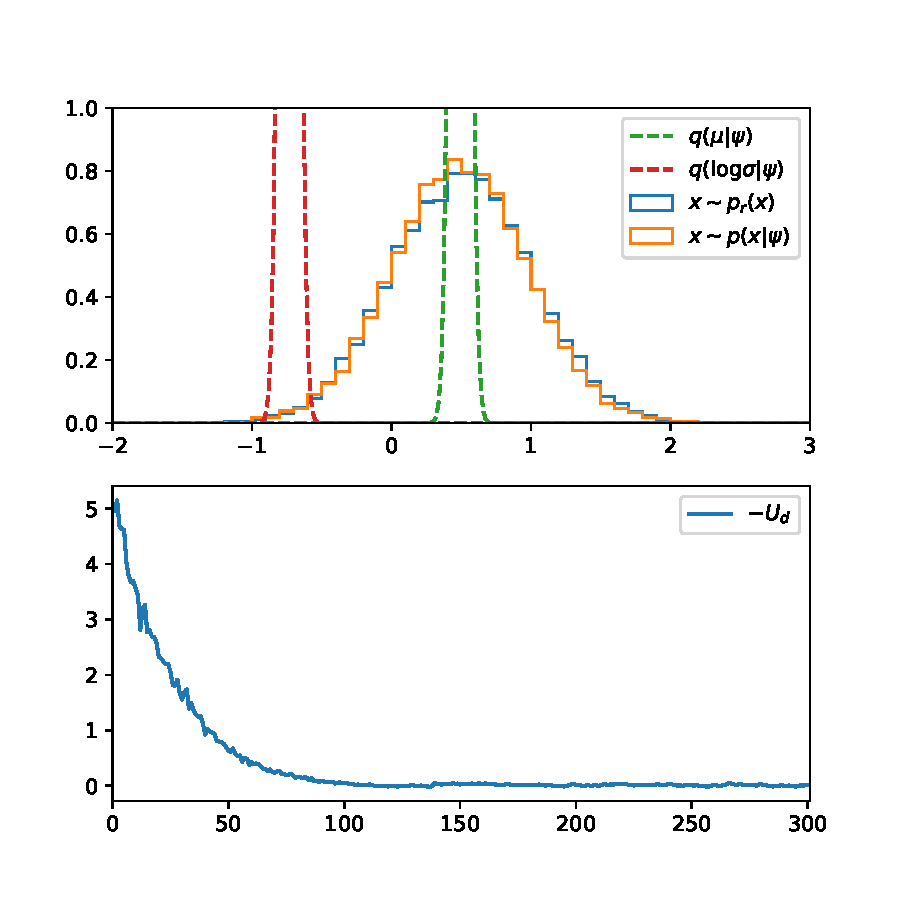
\includegraphics[width=0.48\textwidth]{figures/gaussian-gamma=5.pdf}
    \vspace{-1cm}
    \caption{Toy problem on continuous data: Gaussian with unknown mean and unknown variance.}\label{fig:gaussian}
\end{figure}
\begin{figure}
    \centering
    \vspace{-0.8cm}
    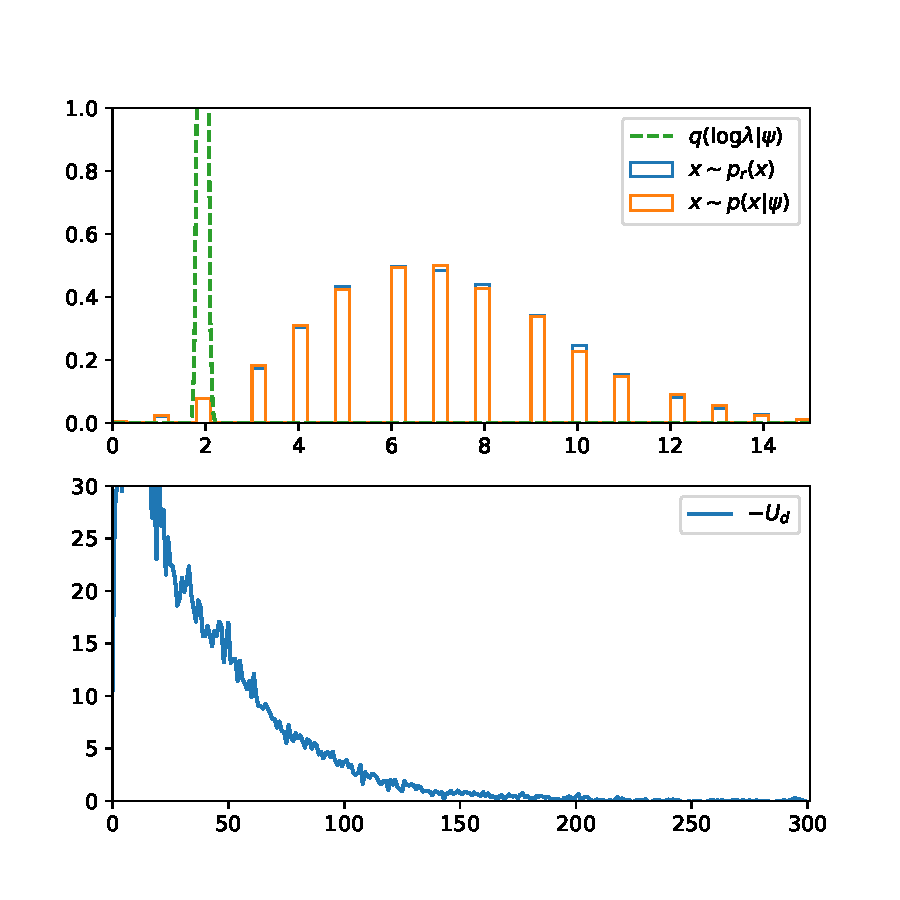
\includegraphics[width=0.48\textwidth]{figures/poisson-gamma=5.pdf}
    \vspace{-1cm}
    \caption{Toy problem on discrete data: Poisson with unknown scale.}\label{fig:poisson}
\end{figure}

The upper plot of Figure~\ref{fig:gaussian} illustrates the resulting model
after the optimization procedure. As expected from adversarial training, the
model density $p(\mathbf{x}|\psi)$ closely matches the true density
$p_r(\mathbf{x})$, as shown by the aligned histograms in blue and orange. Under
the effect of the entropy penalty $\gamma H(q(\theta|\psi))$, we also observe
that the proposal distributions have correctly concentrated their mass around
$\mu=1$ and $\log \sigma=-0.69$. The bottom plot of Figure~\ref{fig:gaussian}
shows an empirical estimate of $-U_d$ with respect to the epoch. We observe
that it quickly falls towards $0$, which indicates that
$\mathbb{E}_{\tilde{\mathbf{x}} \sim p(\mathbf{x}|\theta)} [d(\tilde{\mathbf{x}};\phi)] \approx \mathbb{E}_{\mathbf{x} \sim p_r(\mathbf{x})} [d(\mathbf{x};\phi)]$
and that the critic cannot distinguish between true and model data.

Similarly, we evaluate adversarial variational optimization on discrete data,
for the inference of the scale parameter $\lambda$ of a Poisson distribution.
The observed data is sampled from a univariate Poisson with scale $\lambda=7$.
We use a univariate Gaussian proposal distribution $q(\log \lambda|\psi)$
initialized with a mean at $5$ and unit variance. Hyper-parameters are otherwise
left unchanged with respect to the previous setup. Despite the discreteness
and the non-differentiability of the underlying generator, Figure~\ref{fig:poisson}
shows that inference with adversarial variational optimization works.
The upper plot in the figure shows that $p(\mathbf{x}|\psi)$ closely
matches $p_r(\mathbf{x})$, with the mass of the proposal distribution
concentrated at $\log 7 = 1.94$. 


\subsection{Plinko}



% ==============================================================================

\section{Related works}

As reviewed in \cite{2016arXiv161003483M}, likelihood-free inference is
intimately tied to a class of algorithms that can be framed as density
estimation-by-comparison. In most cases, these inference algorithms are
formulated as an iterative two-step process where the model distribution is
first compared to the true data distribution and then updated to make it more
comparable to the latter.

Closest to our work are procedures that rely on a classifier to estimate the
discrepancy between the true and the model distributions. For example,
\citep{gutmann2012noise} uses non linear logistic regression for fitting
unnormalized differentiable statistical models, while
\citep{goodfellow2014generative} exploits an adversarial neural network for
learning a differentiable implicit generative model. In the likelihood-free
setup, \citep{cranmer2015approximating,2016arXiv161110242D} estimate likelihood
ratios through supervised classification, which can in turn be used for
parameter inference in combination with a gradient-free optimization algorithm.
Similarly, \citep{gutmann2017likelihood} makes use of classification accuracy as
a summary statistics for approximate Bayesian computation.

In this context, the proposed method can be considered as a direct adaptation of
generative adversarial networks~\citep{goodfellow2014generative} to
non-differentiable simulators. It also constitutes an approximate gradient
descent alternative to bayesian optimization based on density
ratios~\citep{cranmer2015approximating} or to classifier
ABC~\citep{gutmann2017likelihood}.


% ==============================================================================

\section{Summary}



% ==============================================================================

\section*{Acknowledgments}

GL and KL are both supported through NSF ACI-1450310, additionally KC is
supported through PHY-1505463 and PHY-1205376.


% ==============================================================================

\bibliographystyle{acm}
\bibliography{bibliography.bib}


\end{document}
